\chapter{Research Methodology}
\label{chp:methodology}
This chapter provides a detailed exposition of the methodology used throughout this work. This study has conducted exploratory and descriptive research to determine whether the use of simulation and an automated feedback driven system, a user can be trained as a race driver. The chapter is structured as follows: \S~\ref{sec:meth-overview} provides a general overview of the overarching methodology used in the study, \S~\ref{sec:meth-experiment-setup} describes in length the design of the instrument used to acquire experiment data and results, \S~\ref{sec:meth-experiment-structure} presents the experimental procedure and the rationale behind it, \S~\ref{sec:meth-data-gathering} identifies the information and data acquired through the experimental and descriptive methodologies employed, and finally \S~\ref{sec:meth-data-analysis} presents the data analysis mechanisms employed to substantiate our conclusions.
%
% Overview
%
\section{Overview}
\label{sec:meth-overview}
This study conducted experimental and descriptive research on the viability of the use of simulators in conjunction with an automated feedback system for improving race driving skills in the normal population. Specifically, a user study was devised and carried out with the primary goals being:
\begin{enumerate}
	\item To determine whether a context-based feedback system can improve the skills of a participant
	\item To quantify the magnitude of this improvement, if (1) is true
\end{enumerate}

These goals were addressed by means of an experimental setup based on a race-driving simulator, using which objective measurement of the participant performance could be gathered and analysed, and a questionnaire for relating the participant's experience with the experimentally-gathered data. The setup of the experiment is explored in more detail in \S~\ref{sec:meth-experiment-setup}.

Since the main goal of this study is that of assessing how effective a feedback system is in the learning process, the independent variable in the experiment is the ability to receive feedback. The hypothesis is that participant performance (such as average lap time) is improved through feedback, and is thus a dependent variable. However, practising without feedback can also lead to changes in the dependent variable; therefore this is controlled for by having two groups of participants: the experimental group that receives feedback and the control group that doesn't. Random assignment is used to determine a participant's group.

A questionnaire, to be administered to the participants at the end of the session, will be designed to help normalise and control for other factors that may influence dependent variables, and hence, the outcome of the experiment. The design of the questionnaire also helps in bridging the participants' perception of their performance with the actual performance data, possibly providing further insight into the results. A questionnaire was preferred to an interview because it is easier to administer, it lends itself to group administration and also allows confidentiality \cite{introductiontobehavioralresearchmethods}.. It is indeed true that interviews permit a greater freedom of expression on behalf of the participant; however, questionnaires create a sense of anonymity that encourages the participants to be more truthful in their answers \cite{introductiontobehavioralresearchmethods}.

\section{Experiment Design}
\label{sec:meth-experiment-design}
In the experiment, each group would be utilising the same car and racetrack. Bastow et al. \cite{bastow2004car} suggest that cars equipped with a front wheel drivetrain may be easier to handle. The Fiat 500 Abarth was the car chosen for the experiments, partially based on Bastow et al.'s findings. The car is relatively low-powered and thus, easier to use by beginning drivers. The Silverstone National race track has the desirable properties of being flat and smooth, without uneven surfaces or bumps which may result in loss of control in rookie drivers. Furthermore, the way the track is structured, with wide run-off areas located along the circuit where drivers are most likely to lose control of the car, allows the car to slow down before colliding with barriers or other stationary objects.

Two feedback mechanisms have been considered for this experiment, \emph{visual}, through the use of a heads-up-display (HUD) superimposed on the simulation display, or \emph{auditory}, by means of descriptive speech projected through loud speakers. Leahy et al. \cite{leahy2003auditory} argue that auditory feedback is less intrusive than visual clues; based on these findings, it was decided that the system should provide feedback using auditory clues.

\begin{figure}
	\centering
	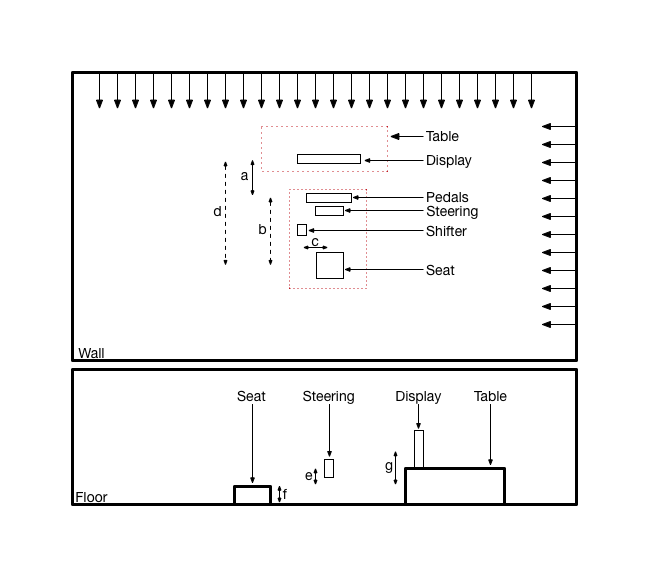
\includegraphics[width=\textwidth]{images/experiment-setup-schematic.png}
	\caption[Experiment Setup Schematic]{Top-down and side views of experiment setup}
	a = 45cm, b = 75cm, c = 36cm, d = 120cm, e = 20cm, f = 30cm, g = 35cm
	\label{fig:meth-experiment-setup}
\end{figure}

\section{Experiment Materials}
\label{sec:meth-experiment-setup}
The setup of the experiment was divided into three material categories: \emph{simulation environment}, \emph{simulation hardware} and \emph{simulation software}, with each category subscribing to a number of desirable properties: 

\begin{description}
	\item [Environment] The experiment should be carried out in an isolated, noise-free and well-lit room. Participants would be let in the room one at a time, to ensure the experiment is conducted without any distractions.
	\item [Hardware] The hardware components identified for this experiment are the (i) display output, (ii) audio output, (iii) steering wheel, (iv) gear shifter, (v) acceleration, brake and clutch pedals and (vi) seating frame.
	\begin{description}
		\item [Display and Audio] A 32"+ display capable of outputting graphics at a progressive resolution of 1080 pixels vertically at 60 Hz (1080p60) is required; smaller display sizes would not yield a large enough solid angle for the participant to feel immersed in the simulator. For audio output, a stereo setup with a speaker output power of 10W should be sufficient; at a distance of 1m, these speakers can generate sound volume up to 100db, where normal conversation is around 60db.
		\item [Driving Controls] The driving controls include (ii)-(iv); minimally a steering wheel should provide the same number of revolutions as a racing car, providing accurate force feedback to let the participants accurately assess the behaviour of the car. Gear shifters do not implement feedback mechanisms; however, given their ubiquity, H-shifters are preferred since they are the kind most drivers are familiar with. High-end pedal systems use hydraulics to simulate the variability of force required on part of the driver to actuate a pedal during different stages.
		\item [Seating Frame] The seating frame should ensure a seating position akin to a driver in a racing car. The seating frame should also provide the ability to move the seat back and forward in order for participants to be able to seat comfortable and be able to reach the pedals.
	\end{description}
	\item [Software] The software aspect of the experiment, which is primarily the racing simulator, should have a number of desirable properties. In particular, the simulator should provide (i) a realistic driving model, (ii) driving aid customisation, (iii) high-fidelity graphics, (iv) real-world tarmac circuits, (v) and telemetry data access through an interface that is intuitive to use.
	\begin{description}
		\item [Realistic Driving Model] For this experiment, a realistic driving model is a sine qua non. Recreating real-world conditions requires a high-fidelity physics simulation of race car dynamics that is as close to the real thing as possible.
		\item [Driving Aid Customisation] Required to control experiment variables, such as tyre wear and tear. The aim is to prevent car behaviour from changing as the experiment progresses. 
		\item [High-fidelity Graphics] Required to provide the participant with a fully immersive experience.
		\item [Real-world Tarmac Circuits] Most racing simulators accurately replicate real-world tracks, up to minute details such as elevation changes and bumps. This level of realism exposes participants to real-life scenarios. Furthermore, the simulator should provide circuits that loop, to streamline experiments and remove the need to reset the software in order to drive another lap.  
		\item [Telemetry Data Access] The premise of this project hinges on the ability to read telemetry data from a simulator. Thus, any software that does not provide this feature is a priori discarded. However, easier and cleaner interfaces for reading telemetry data, and the breadth of telemetry data offered, are a deciding factor in the choice of racing simulator to use.
	\end{description}
\end{description}

\subsection{Hardware Selection}
A number of racing simulator input devices have been considered (see Table \ref{tab:racing-input}). The choice was narrowed down to the most popular devices among racing game enthusiasts, the Logitech G25~\cite{logitecg25}, the Thrustmaster TX~\cite{TrustmasterTX} and the Fanatec CS~\cite{Fanatec}. The G25 provides the minimally required features: a steering wheel with a $900\degree$ turn, 3-pedal set, H-shifter and force feedback; furthermore, the G25 is also a very affordable device. Both the Thrustmaster and Fanatec are high-end devices, which explains the cost difference. Furthermore, neither come with the 3-pedal set and the H shifter, which have to be purchased separately. The Logitech G25 was chosen for being the most cost-effective of the three options.

\begin{table}[htb!]
    \centering
    \begin{tabular}{lccccc}
        \toprule
        \textbf{Device} & \textbf{$900\degree$} & \textbf{3-Pedal Set} & \textbf{H-Shifter} & \textbf{Feedback} & \textbf{Cost} \\
        \midrule
        Logitech G25 & \checkmark & \checkmark & \checkmark & Low & 240 \\
        Thrustmaster TX & \checkmark & & & Med & 324 \\
        Fanatec CS & \checkmark & & & High & 850 \\
		\bottomrule		
	\end{tabular}
	\caption{Comparison of input devices}
	\label{tab:racing-input}	
\end{table}

\subsection{Software selection}
Similarly to the hardware selection process, a number of racing simulators have been considered (see Table \ref{tab:sim-choice}). Although there is a myriad of racing simulators available, the selection process narrowed them down to a popular handful: Forza Motorsports 6 \cite{forza} by Turn 10 Studios, Project Cars\cite{ProjectCars} by Slightly Mad Studios, Assetto Corsa\cite{assestoCorsa} by Kunos Simulazioni, iRacing\cite{iRacing} by iRacing.com Motorsports Simulations and Dirt \cite{dirtgame} by Codemasters. Unfortunately, notwithstanding its quality, Forza Motorsports 6 does not provide access to telemetry information. Dirt also suffers from the same shortcoming, in addition to providing very little in terms of track applicability: very few tracks are circuit-based. iRacing provides most of the functionality required by the experiment, however in terms of visual quality it suffers when compared to Project Cars and Assetto Corsa. Finally, the choice between Assetto Corsa and Project Cars was made on the basis of ease of interfacing for the acquisition of telemetry data; here we felt Assetto Corsa provided a clean, intuitive and ultimately superior interface to telemetry acquistion via User Datagram Protocol (UDP) connections.

%The comparison table shows the desired properties a sim game must have, and a selection of games which have been considered. From the start it is clear, Dirt and Forza 6 should be discarded as none provide telemetry data to be read. Assetto Corsa, Project Cars and iRacing are closely matched, however Assetto Corsa has the leading edge as it provides an easy way to interface via UDP, well document and wide developer community who can help. Furthermore Assetto Corsa provides good visual graphics. For these reasons Assetto Corsa has been picked as the sim to be used.

\begin{table}[htb!]
    \centering
    \begin{tabular}{lcccccc}
        \toprule
        \textbf{Simulator} & 
        \multicolumn{1}{p{1.2cm}}{\centering \textbf{Driving} \\ \textbf{Model}} &
        \multicolumn{1}{p{1.2cm}}{\centering \textbf{Driving} \\ \textbf{Aids}} &
        \multicolumn{1}{p{1.2cm}}{\centering \textbf{Visual} \\ \textbf{Quality}} &
        \multicolumn{1}{p{1.1cm}}{\centering \textbf{Tracks}} &
        \multicolumn{1}{p{1.1cm}}{\centering \textbf{Tele-metry}} &
        \multicolumn{1}{p{1.1cm}}{\centering \textbf{I/F Ease}} \\
        \midrule
        Forza & \checkmark & \checkmark & \checkmark & \checkmark & & \\ 
        Project Cars & \checkmark & \checkmark & \checkmark & \checkmark & \checkmark & \\ 
        Assetto Corsa & \checkmark & \checkmark & \checkmark & \checkmark & \checkmark & \checkmark \\ 
        iRacing & \checkmark & \checkmark & & \checkmark & \checkmark & \checkmark \\ 
        Dirt & \checkmark & \checkmark & \checkmark & & & \\ 
		\bottomrule		
	\end{tabular}
	\caption[Comparison of Racing Simulators]{Comparison of racing simulators on the basis of a realistic driving model, customisable driving aids, high-fidelity graphics quality, applicability of tracks, availability of telemetry information, and ease of interfacing.}
	\label{tab:sim-choice}	
\end{table}

%
%\begin{center}
%	\begin{tabular}{ | l | l | l | l | l | l |}
%		\hline
%			& Assetto Corsa\cite{assestoCorsa} & pCars \cite{ProjectCars} & iRacing \cite{iRacing} & Dirt \cite{dirtgame} & Forza 6 \cite{forza} \\ \hline
%		Realistic model	& \checkmark &\checkmark & \checkmark & \checkmark & \checkmark \\ \hline
%		Tracks	& \checkmark &\checkmark & \checkmark &  & \checkmark \\ \hline
%		Disable wear & \checkmark & \checkmark & \checkmark & \checkmark & \checkmark \\ \hline
%		Telemetry data	& \checkmark & \checkmark & \checkmark &  &  \\ \hline
%		Ease of Interfacing	& \checkmark &  & \checkmark &  &  \\ \hline
%		Quality of graphics & \checkmark & \checkmark &  & \checkmark & \checkmark \\ \hline
%	\end{tabular}
%\end{center}

\subsection{Participant Information and Feedback}
Questionnaires are a very important tool for acquiring insight from the point of view of experiment participants, and when compared to interviews, they provide a framework within which respondents can answer more truthfully due to lack of social external pressures. Leary et al. \cite{introductiontobehavioralresearchmethods} provide a set of guidelines for compiling questionnaires, consisting of seven general rules:
\begin{enumerate}
	\item Be specific and precise in phrasing the questions;
	\item Write the questions as simply as possible, avoiding difficult words, unnecessary jargon, and cumbersome phrases;
	\item Avoid making unwarranted assumptions about the respondents;
	\item Conditional information should precede the key idea of the question;
	\item Do not use double-barrelled questions;
	\item Pretest the questions.
\end{enumerate}
Responses from questionnaires designed using these guidelines are valid in the general case. A further challenge posed by questionnaire compilation is that of choosing a response format for each question: open-ended questions may serve to collect more information but be less conducive to analysis, while on the other hand, more restrictive and constrained response formats may lack expressivity but be easier to analyse. Leary et al. suggest using constrained response formats, such as the Likert scale \cite{likert1932technique}, when dealing with behaviours, thoughts or feelings that can vary in frequency or intensity, and open-ended questions in cases where further insight is desired. 

Two qualitative questionnaires have been designed in accord with these guidelines, one with the aim of gathering insight into the participant demographics, and a second to help normalise and control for factors that may influence dependent variables, to bridge the participants' perception of their performance with the actual execution, and to gather other insight and feedback about the experiment.

%A questionnaire, to be administered to the participants at the end of the session, will be designed to help normalise and control for other factors that may influence dependent variables, and hence, the outcome of the experiment. The design of the questionnaire also helps in bridging the participants' perception of their performance with the actual performance data, possibly providing further insight into the results.

%The challenge in choosing a response format in a question lies in identifying whether one should go for an open ended question in which more information might be collected, or on the other hand, use a rating scale response format, where the response is more constrained but may be easier to analyse. Leary et al. suggest using the former for questions dealing with behaviours, thoughts, or feelings that can vary in frequency or intensity (e.g. the Likert Scale\cite{likert1932technique}) and using open ended questions in cases where further insight is desired.

%Based on these guidelines two qualitative questionnaires have been designed, one aiming to gather insight into the sample demographic, the other aiming to gain insight into the participants' impressions about the realism of the experiment setup, the level of comfort, or discomfort and any suggestions or comments they might have. 

%\subsection{Participant Demographic}
%
%\subsection{Participant Feedback}

\section{Experiment Procedure}
\label{sec:meth-experiment-structure}
In this section, we describe in detail the experiment procedure. Participants are gathered through various methods, ranging from word-of-mouth to mailing lists, where each participant would reserve an experiment time slot. Participants are split randomly into two groups. The first group is referred to as the \emph{feedback group}, the second as the \emph{control group}. 

%In order to evaluate the effectiveness of the system a user study took place. Participants were split randomly into two groups. One group will be referred as the feedback group, the other will be referred to as the base group. The experiments structure was subdivided into smaller systemic tasks.

\begin{description}
	\item[Introduction] Each participant is introduced to the setup and given an overview of the experiment procedure. 

	\item[Demographic Questionnaire] The experiment starts by the participant responding to a brief questionnaire, aimed to gather more insight about the general participant demographics.
	
	\item[Rig Configuration] 
	The user climbs inside the rig; the seating position is adjusted to accommodate the user, making sure he or she is sitting comfortably, and all controls can be reached with ease. Participants are given a second, more in-depth overview of the components of the rig and how they operate. This explanation covers the steering wheel, the pedal layout and function and the H-shifter.
	
	\item[Practice (10 minutes)] The participant is given ten minutes to get used to the rig setup, track and car. This session is aimed at gauging the skill level of the user while he or she gets acquainted with the simulator.
	
	\item[Break (5 minutes)] A short break (5 minutes maximum) is given to each participant.
	
	\item[$1^{st}$ Session (10 minutes)] In this session, the participant drives the racing car around the track for ten minutes. Participants in the feedback group have the feedback system turned on, while for the control group, this is turned off.
	
	\item[Break (5 minutes)] A short break (5 minutes maximum) is given to each participant.

	\item[$2^{nd}$ Session (10 minutes)] A second ten minute session is held; participants in the feedback group have the feedback system turned on, while for the control group, this is turned off.
	
	\item[Break (5 minutes)] A short break (5 minutes maximum) is given to each participant.
	
	\item[$3^{rd}$ Session (5 minutes)] A final five minute driving session; the feedback system is turned off for participants in both groups. This session was included to help identifying conclusive results about the feedback system and its effects on the participants. 
	
%	\item[Five minuties session] A final five minuties of driving are allocated yet again, this time with the feedback system turned of for both groups. This was designed to possibly identify any conclusive results. Such session could show the possibility of the feedback group performing worst after having the aid of the feedback system removed or both groups ending up performing the same after the sessions, which would suggest the feedback participant didn't manage to get any cognitive advantage.
	
	\item[Feedback Questionnaire] The experiment concludes by the participant responding to a questionnaire about experiment structure, apparatus quality, performance perception and free-form participant feedback.
	
%	\item[Particpant's feedback questionare] The final stage of the experiment requires participants to fill in the a questionnaire  in which they are asked to give their feedback on the experiment structure, hardware used and any further comments they would like to add.
	
\end{description}

\section{Data Collection and Sampling}
\label{sec:meth-data-gathering}
At the end of the experiments the data collected includes two questioners from each participant and four batches of telemetry data, one for each participant. Questioners are filled online using Google Forms as it provides the ability to export the data and also automatic generation of descriptive statistic. The data collected from the questionnaires and telemetry data is to be loaded into a data base management system from which the data can be queried using specialised data querying constructs. By having a querying language, it provides the flexibility of extracting data which is relevant for the data analysis at hand.

\section{Data Analysis}
\label{sec:meth-data-analysis}
In order to accept or reject the null hypothesis statistical test are to be carried out. Most important is the ability to compare the performance of the two groups across sessions. The lap time is used as the test variable as this gives a good indication for the average performance achieved during a lap. Furthermore which comparison test to use depends on the sample size, the distribution of data and the types of group. In this case the groups are independent from each other, as a participant may not be part of the base group and also part of the feedback group. As pointed out by De Smith in his book "Statistical Analysis Handbook-a web-based statistics" the tests of interest to this project are the Independent samples t-test\cite{de2015statsref} and the Mann Whitney U test\cite{de2015statsref} as these test for difference between independent groups. Both tests share the same hypothesis listed below.

\begin{description}
	\item[Independent t test] assumes the data is normally as such the data must be checked for normal distribution. This can be carried out by using the Shapiro-Wilk\cite{de2015statsref} test for normality on both groups.
	
	\item[Mann Whitney U test] Does not require the data to be normally distributed however, it assumes the groups' data shares the same distribution. The groups are checked for equal distribution using the Independent Samples Kolmogorow-Smimov test.
	
	\item[Null hypotesis]there is no significant difference across the groups
	\item[Alternative hypotesis]there is significant difference across the groups
\end{description}

As the data distribution is not known before hand, distribution tests will be carried out after the data is collected and depending on the result, the adequate test will be used.